%FILL IN THE RIGHT INFO.
%\lecture{**LECTURE-NUMBER**}{**DATE**}
\unchapter{Lecture 2}
\lecture{2}{September 8}
\setcounter{section}{0}
\setcounter{theorem}{0}
% **** YOUR NOTES GO HERE:

\section{Complex Power Series}

\begin{definition}
Consider a sequence $\{a_n\}_{n=0}^\infty \subset \mathbb{C}$. Then the \textbf{complex series} defined by this sequence is $\sum_{n=0}^\infty a_nz^n \in \C$.
\end{definition}

\begin{proposition}
Given a power series $f(z)=\sum_{n=0}^\infty a_nz^n$ then $\exists R \in [0,\infty]$ such that
\begin{enumerate}
    \item If $\abs{z}<R$ then $f(z)$ converges absolutely (i.e. $\sum_{n=0}^\infty \abs{a_n}\abs{z}^n < \infty$),
    \item If $\,\abs{z}>R$ then $f(z)$ diverges.
\end{enumerate}
Furthermore:
\begin{align*}
    R=\frac{1}{\limsup\limits_{n\rightarrow \infty} \, \abs{a_n}^\frac{1}{n}}.
\end{align*}
This R is called the radius of convergence of $f(z)$.
\end{proposition}

\begin{proof}
Let $L=\limsup\limits_{n\rightarrow \infty} \, \abs{a_n}^\frac{1}{n}$. Assume $0<L<\infty$. Let $R=\frac{1}{L}$.
\begin{enumerate}
    \item Suppose $\abs{z}<R=\frac{1}{L}$. Since the inequality is strict $\exists \varepsilon>0$ s.t. $r\vcentcolon=(L+\varepsilon)\abs{z}<1$. By definition $\abs{a_n}^\frac{1}{n}\leq L+\varepsilon$ for large $n$. Then:
    \begin{align*}
        \abs{a_n} \abs{z}^n &\leq \br{\br{L+\varepsilon}\abs{z}}^n = r^n\\
        &\Downarrow\\
        \sum_{n=0}^N \abs{a_n}\abs{z}^n &\leq \sum_{n=0}^N r^n \leftarrow \text{converges}.
    \end{align*}
    \item Suppose $\abs{z}>R$. Choose $\varepsilon>0$ s.t. $r\vcentcolon=(L-\varepsilon)\abs{z}>1$. By definition $\exists n_j$ s.t. $\big|a_{n_j}\big|^\frac{1}{n_j}> (L-\varepsilon) \,\,\, \forall j$. Hence: 
    \begin{align*}
        \big|a_{n_j}\big|\abs{z}^{n_j} &\geq ((L-\varepsilon)\abs{z})^{n_j} = r^{n_j}\\
        &\Downarrow\\
        \sum_j \big|a_{n_j}\big|\abs{z}^{n_j} &\geq \sum_j r^{n_j} \leftarrow \text{diverges}.
    \end{align*}
\end{enumerate}
And we are done.
\end{proof}

\begin{theorem}\label{thm:power-series-implies-CR}
Let $f(z)= \sum_{n=0}^\infty a_n z^n$ with $R_f = R>0$. Let $D_R = D_R(0) = \set{z\in \mathbb{C} : \abs{z}<R }$. Then $f(z)$ is holomorphic on $D_R$, with $f'(z)= \sum_{n=1}^\infty na_n z^{n-1}$ and $R_{f'} = R_f$.
\end{theorem}

\begin{proof}
Let $g(z) = \sum_{n=1}^\infty na_n z^{n-1}$. Then $R_g=R_f$ since:
\begin{align*}
    \limsup\limits_{n\rightarrow \infty} \, \abs{na_n}^\frac{1}{n-1} &= \limsup\limits_{n\rightarrow \infty} \, \big( \, \abs{na_n}^\frac{1}{n}\big)^{\frac{n}{n-1}}\\
    &= \limsup\limits_{n\rightarrow \infty} \, \big( \, \cancelto{1}{\abs{n}^\frac{1}{n}}\abs{a_n}^\frac{1}{n}\big)^{\cancelto{1}{\frac{n}{n-1}}} = \limsup\limits_{n\rightarrow \infty} \, \abs{a_n}^\frac{1}{n}.
\end{align*}

Given $z_0 \in D_R$ choose $r>0$ s.t. $\abs{z_0}<r<R$. Then for every $N\geq 1$ let:
\begin{align*}
    S_N(z) &= \sum_{n=0}^N a_nz^n \leftarrow \text{converges}\\
    E_N(z) &= \sum_{n=N+1}^\infty a_nz^n \leftarrow \text{converges on $D_R$}
\end{align*}
Then $f(z) = S_N(z)+E_N(z)$ on $D_R$. If $h$ is such that $\abs{z_0+h}<r$, then
\begin{align*}
    \frac{f(z_0+h)-f(z_0)}{h} - g(z_0)
    & = \frac{S_N(z_0+h)-S_N(z_0)}{h} - S_N'(z_0)&& \circled{1} \\& +S_N'(z_0)-g(z_0)&& \circled{2} \\& +\frac{E_N(z_0+h)-E_N(z_0)}{h} && \circled{3}
\end{align*}

We now show that for large $N$, these lines all go to zero.

\begin{itemize}
    

    \item[\circled{3} :]
    \begin{align*}
        \abs{\frac{E_N(z_0+h)-E_N(z_0)}{h}} &\leq \sum_{n=N+1}^\infty \abs{a_n} \underbrace{\abs{\frac{(z_0+h)^n-z_0^n}{h}}}_{a^n-b^n=(a-b)(a^{n-1}+\cdots+b^{n-1})}\\
        &= \sum_{n=N+1}^\infty \abs{a_n} \abs{\frac{(z_0+h-z_0)((z_0+h)^{n-1}+\cdots+(z_0)^{n-1})}{h}}\\
        &\leq \sum_{n=N+1}^\infty \abs{a_n} \abs{\frac{h(r^{n-1}+\cdots+r^{n-1})}{h}} = \sum_{n=N+1}^\infty \abs{a_n} \big|nr^{n-1}\big|.
    \end{align*}
    This is the tail of the power series $g(z)$, but we know that $g(z)$ converges absolutely on $D_R$. Thus:
    \begin{align*}
        \abs{\frac{E_N(z_0+h)-E_N(z_0)}{h}} \leq \sum_{n=N+1}^\infty \abs{a_n} \big|nr^{n-1}\big| \xrightarrow[]{N \to \infty} 0.
    \end{align*}
    
    \item[\circled{2} :]
    \begin{align*}
        \abs{S_N'(z_0)-g(z_0)} &=\abs{\sum_{n=1}^N na_n z_0^{n-1} -\sum_{n=1}^\infty na_n z_0^{n-1}}\\
        &= \abs{\sum_{n=N+1}^\infty na_n z_0^{n-1}}
    \end{align*}
    which goes to 0 for big N.
    
    \item[\circled{1} :] Note that $S_N(z)$ is holomorphic at $z=z_0$, as it is a polynomial. Thus:
    \begin{align*}
        \frac{S_N(z_0+h)-S_N(z_0)}{h} - S_N'(z_0) \rightarrow 0
    \end{align*}
    
\end{itemize}

Combining these three points, we see that for $N$ sufficiently large,
\begin{align*}
    \abs{\frac{f(z_0+h)-f(z_0)}{h} - g(z_0)} \rightarrow 0,
\end{align*}
and we are done.
\end{proof}



\begin{corollary}
A power series with $R>0$ is infinitely many times complex differentiable on the disk $D_R$, and the higher derivatives are obtained by term-wise differentiation of the elements in the power series.
\end{corollary}

\begin{remark}
We can consider power series centered at some point $z_0\in\mathbb{C}$ (until now we have been considering the special case $z_0 = 0$) with the form:
\begin{align*}
    f(z)&=\sum_{n=0}^\infty a_n(z-z_0)^n\\
    \text{with } f'(z)&=\sum_{n=1}^\infty na_n(z-z_0)^{n-1}\\
    & \ \vdots
\end{align*}

This has the same radius of convergence as you would expect, but it is convergent on $D_R(z_0)=\set{z\in \mathbb{C} : \abs{z-z_0}<R }$.
\end{remark}

\begin{example}[Geometric Power Series] A standard example of a power series is:
\begin{align*}
    f(z)&=\sum_{n=0}^\infty z^n ,\\
    \rightarrow R&= 1, \\
    f(z_0)&=\sum_{n=0}^N (z_0)^n = \frac{1-z_0^{N+1}}{1-z_0} \xrightarrow{N\rightarrow\infty} \frac{1}{1-z_0}.
    \end{align*}
\end{example}

\begin{example}[Exponential Power Series] A second standard power series is:
\begin{align*}
    e^z&\defas \sum_{n=0}^\infty \frac{z^n}{n!} , \\
    R&= \infty.
\end{align*}
$e^z$ is a holomorphic function on $\mathbb{C}$. Clearly if $x\in\mathbb{R}\subset\mathbb{C}$ then $e^x$ is the usual exponential function. Note that:
\begin{align*}
    (e^z)' &= \left( \sum_{n=0}^\infty \frac{z^n}{n!} \right)'= \sum_{n=1}^\infty \frac{\cancel{n}\cdot z^{n-1}}{\cancel{n}\cdot (n-1)!}= \sum_{n=0}^\infty \frac{z^n}{n!}= e^z.
\end{align*}
Further note that:
\begin{align*}
    e^{z+w} = e^z\cdot e^w.
\end{align*}
\end{example}

\section{Properties of $e^z$}
We now consider some interesting aspects of the function $e^x$.
\subsection{Definition of $\cos(z)$ and $\sin(z)$}

Consider $\theta \in \mathbb{R}$. Then it is a well-known fact that:
\begin{align*}
    e^{i\theta}&=\sum_{n=0}^\infty \frac{(i\theta)^n}{n!}\\
    &= \underbrace{\left( \sum_{n=0}^\infty (-1)^n \frac{\theta^{2n}}{(2n)!}  \right)}_{\cos(\theta)} + i \cdot \underbrace{\left( \sum_{n=0}^\infty (-1)^n \frac{\theta^{2n+1}}{(2n+1)!}  \right)}_{\sin(\theta)}\\
    &= \cos(\theta)+i\sin(\theta).
\end{align*}

\begin{remark}
If $z\neq0$, let $\theta = \arg(z)$. Then $z=\abs{z}\cdot e^{i\theta}$.
\end{remark}

\begin{remark}
Consider now the function $e^{iz}, \, z\in\mathbb{C}$. Then:
\begin{align*}
    e^{iz}&=\underbrace{\left( \sum_{n=0}^\infty (-1)^n \frac{z^{2n}}{(2n)!}  \right)}_{=\vcentcolon \, \cos(z)} + i \cdot \underbrace{\left( \sum_{n=0}^\infty (-1)^n \frac{z^{2n+1}}{(2n+1)!}  \right)}_{=\vcentcolon \, \sin(z)}.
\end{align*}

The functions $\cos(z)$ and $\sin(z)$ are both holomorphic functions $\forall z \in \mathbb{C}$, which gives us the complex version of Euler's formula:
\begin{equation*}
e^{iz} = \cos(z) + i\sin(z)\\
\end{equation*}
Note that:
\begin{align*}
    \cos(-z) &= \cos(z)\\
    \sin(-z) &= -\sin(z)\\
    &\Downarrow\\
    e^{-iz} &= \cos(z) - i\sin(z)\\
    &\Downarrow\\
    \cos(z) &= \frac{e^{iz}+e^{-iz}}{2}\\
    \text{and } \sin(z) &= \frac{e^{iz}-e^{-iz}}{2i}
\end{align*}
\end{remark}

\begin{definition}[Analytic Functions]
$\Omega \subset \mathbb{C}$ a domain, $f:\Omega \rightarrow \mathbb{C}$. We say that $f$ is \textbf{analytic} (on $\om$) if $\forall z_0 \in \Omega$, $\exists r>0$ s.t. $D_r(z_0) \subset \Omega$ and $\exists \{ a_n  \}_{n=0}^\infty \subset \mathbb{C}$ s.t. $f(z) = \sum_{n=0}^\infty a_n (z-z_0)^n$ and this power series converges absolutely on $D_r(z_0)$ (i.e. $f(z)$ is analytic if locally it is equal to an absolutely convergent power series).
\end{definition}

\begin{remark}
Since power series are holomorphic, then $f(z)$ analytic on  $\Omega$ $\implies$ $f(z)$ holomorphic on $\Omega$. 
\end{remark}

\begin{theorem}
Holomorphic functions are analytic.
\end{theorem}

\begin{proof}
To be done in a following lecture.
\end{proof}

\begin{remark}
This is one way in which complex analysis veers away from real analysis. This theorem is not true in real analysis; there is a big gap between differentiable and analytic in $\mathbb{R}$, but none in $\mathbb{C}$.
\end{remark}

\section{Contour/Line Integrals}
A contour integral is an integral of a function along a curve.

\subsection{Parameterized Curves in $\mathbb{C}$}

Consider a function $\gamma:[a,b] \rightarrow \mathbb{C}$ with $[a,b] \subset \mathbb{R}$. We assume that $\gamma(t)$ is at least piece-wise smooth. We often write $\gamma(t)=z(t)$ with $t\in [a,b]$.


\begin{definition}[Piece-Wise Smooth]
A function $\gamma [a,b] \rightarrow \mathbb{C}$ is called \textbf{piece-wise smooth} if $\exists a=a_0<a_1< \cdots < a_N = b$ such that $\gamma(t)$ is continuous on $[a,b]$, and that $\gamma(t)$ restricted to $[a_j,a_{j+1}]$ is infinitely differentiable with $\gamma'(t)\neq 0$ $\forall t\in [a_j,a_{j+1}]$.
\end{definition}

\begin{center}

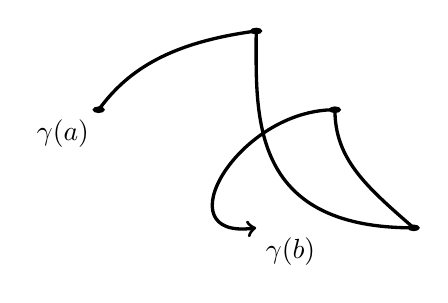
\begin{tikzpicture}[yscale=0.5]

\draw[very thick] (0,0) to [out=70,in=195] (2,2);
\draw[very thick] (2,2) to [out=270,in=180] (4,-3);
\draw[very thick] (4,-3) to [out=120,in=270] (3,0);
\draw[very thick][->](3,0) to [out=180,in=195] (2,-3);


\draw[fill] (0,0) circle [radius=2pt];
\draw[fill] (2,2) circle [radius=2pt];
\draw[fill] (4,-3) circle [radius=2pt];
\draw[fill] (3,0) circle [radius=2pt];
\node[below left] at (0,0) {$\gamma(a)$};
\node[below right] at (2,-3) {$\gamma(b)$};

\end{tikzpicture}

\textit{An example of a piece-wise smooth function.}
\end{center}


\begin{example}[CCW Circle]
Let $z(t) = z_0+e^{it}$. This traces a circle in $\mathbb{C}$.
\end{example}

\subsection{Reparameterization of Curves}

\begin{definition}[Reparameterization]
A \textbf{reparameterization} of a curve $\gamma(t)$ is a function $\Tilde{\gamma}(s) = \gamma(t(s))$ where $s\in[c,d]$ and the map  $s \mapsto t(s)$ is a smooth and strictly increasing bijection $[c,d] \rightarrow [a,b]$. The map $s \mapsto t(s)$ is called the change of parameter from the interval [c,d] to [a,b]. 
\end{definition}

\begin{note}
The mapping must be strictly increasing to ensure that the initial point of the first curve is the same as the initial point of the second curve, and the same with the end points. The curve can however be inverted:
\end{note}

\begin{example}
Consider $\gamma(b+a-t) = \Tilde{\gamma}(t)$. This reverses the direction of the curve.
\end{example}


\begin{center}

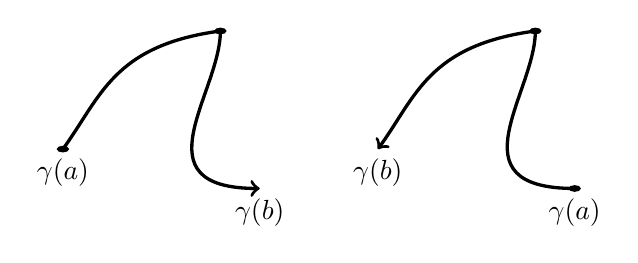
\begin{tikzpicture}[yscale=0.5]

\draw[very thick] (0,0) to [out=70,in=195] (2,3);
\draw[very thick][->] (2,3) to [out=270,in=180] (2.5,-1);
\draw[fill] (0,0) circle [radius=2pt];
\draw[fill] (2,3) circle [radius=2pt];
\node[below] at (0,0) {$\gamma(a)$};
\node[below] at (2.5,-1) {$\gamma(b)$};


\draw[very thick][<-] (4,0) to [out=70,in=195] (6,3);
\draw[very thick] (6,3) to [out=270,in=180] (6.5,-1);
\draw[fill] (6.5,-1) circle [radius=2pt];
\draw[fill] (6,3) circle [radius=2pt];
\node[below] at (6.5,-1) {$\Tilde{\gamma}(a)$};
\node[below] at (4,0) {$\Tilde{\gamma}(b)$};

\end{tikzpicture}

\textit{An example of a curve and its reversed equivalent.}
\end{center}


\begin{example}[CW circle]
Consider the parameterization $z(t) = z_0+e^{it}$ of a circle. The reparameterization $\Tilde{z}(t) = z_0+e^{-it}$ is the same circle but traced CW.
\end{example}

\subsection{Contour Integrals}
\begin{definition}[Contour Integral]
Given a parameterized (parameterized by $z(t)$) curve $\gamma(t)$ s.t. $\gamma([a,b]) \subset \Omega \subset \mathbb{C}$, and a continuous function $f:\Omega \rightarrow \mathbb{C}$, we define the \textbf{contour integral of $f(z)$ over $\gamma$} as:
\begin{align*}
    \int_{\gamma} f(z)  \dif z & \vcentcolon= \int_a^bf \br{z\br{t}} \cdot z'\br{t} \,  \dif t \in \mathbb{C}
\end{align*}
if $\gamma$ is smooth. If it is only piece-wise smooth, then:
\begin{align*}
    \int_{\gamma} f(z)  \dif z & \vcentcolon= \sum_{j=0}^{N-1} \int_{a_j}^{a_{j+1}}f\br{z\br{t}} \cdot z'\br{t} \,  \dif t \in \mathbb{C}.
\end{align*}

\end{definition}


For now a contour integral is a 'black box' which takes in a parameterized curve $\gamma$ and a complex function $f(z)$ and outputs a complex number. It has some nice properties that come along with it:

\begin{itemize}
    \item The value of the integral is not dependant on the parameterization.
    \begin{align*}
        \int_{\gamma} f(z)  \dif z &= \int_a^bf(z(t)) \cdot z'(t) \,  \dif t\\
        &= \int_c^d f(z(t(s))) \cdot \underbrace{z'(t(s)) \cdot t'(s)}_{\Tilde{z}'(s) \text{ by chain rule}} \,  \dif s\\
        &= \int_c^df(\Tilde{z}(s)) \cdot \Tilde{z}'(s) \,  \dif s.
    \end{align*}
\end{itemize}

More properties will come in future lectures.

